\documentclass[10pt,a4paper]{article}
\usepackage[T1]{fontenc}
\usepackage[utf8]{inputenc}
\usepackage{lmodern}
\usepackage[margin=22mm]{geometry}
\usepackage{microtype}
\usepackage{graphicx}
\usepackage{booktabs}
\usepackage{tabularx}
\usepackage{array}
\usepackage{xcolor}
\usepackage{listings}
\usepackage{tikz}
\usetikzlibrary{positioning,arrows.meta,fit,backgrounds}
\usepackage[font=small,labelfont=bf]{caption}
\usepackage{subcaption}
\usepackage{enumitem}
\usepackage[hidelinks]{hyperref}

\setlist{itemsep=1pt,topsep=3pt}
\newcommand{\code}[1]{\texttt{#1}}
\definecolor{codebg}{gray}{0.96}
\lstset{basicstyle=\ttfamily\footnotesize,backgroundcolor=\color{codebg},frame=none,
  columns=fullflexible,keepspaces=true,showstringspaces=false,xleftmargin=4pt,xrightmargin=4pt,
  aboveskip=6pt,belowskip=6pt,commentstyle=\color{black!55},keywordstyle=\bfseries}

\title{\textbf{Emulating a Synthesizer Before It Arrives}\\[2pt]
\large Recovering an undocumented CPU from its firmware and running the M-VAVE FM-1\\ in a browser}
\author{Joakim Eriksson\\\small\url{https://github.com/joakimeriksson/fm1-emu}}
\date{Technical report \quad\textperiodcentered\quad 13 October 2026, with Section~\ref{sec:hw} on the real hardware added 24 October and extended 26 October 2026}

\begin{document}
\maketitle

\begin{abstract}
\noindent
The M-VAVE FM-1 is a pocket FM synthesizer for which a small community writes its own firmware.
It is built on a JieLi AC791N, a dual-core system-on-chip whose CPU, pi32v2, has no public
instruction-set manual. This report describes, step by step, how an emulator of the whole
instrument was built in five days, before the physical unit had been delivered: recovering the
instruction set from vendor disassembly of 25 firmware images, solving operand encodings as exact
linear models, validating semantics with differential probes in which the vendor compiler's own
constant folding is the oracle, modelling the peripherals the firmwares actually touch, and making
it fast enough for real time with two just-in-time compilers (AArch64 natively, WebAssembly in the
browser). The emulator runs M-VAVE's stock firmware on both cores and fifteen community firmwares
unmodified, takes MIDI in, and is published as a web page. Every performance change was accepted
only if the emulated audio stayed byte-identical across three execution modes. The emulator was
then used as the development platform for a new firmware, \emph{FM-1 SID}, which runs a Commodore~64
tune's 6502 code and a reSID model of the SID chip on the FM-1's CPU. The work was done by one person
directing an AI coding agent; the report closes with how that collaboration was organised and which
rules made its output trustworthy. A section added once the hardware arrived tells what releasing
FM-1 SID before anyone had run it on an FM-1 cost its first users, and how it was made to work on the
device in four rounds. Their tool is \emph{fm1-dock}, a host firmware installed once, through which
synths are deployed and probes are run from RAM. The probes compare the emulator with the real FM-1,
and their findings changed the emulator: CPU guards, LCD timing, a measured cycle and flash-cache
model, and a survey of what 80 firmwares execute.
\end{abstract}

\section{Introduction}

The M-VAVE FM-1 (Fig.~\ref{fig:page}) is a battery-powered six-operator FM synthesizer with a
240$\times$240 colour screen, 27 keys, 14 buttons, 7 encoders, a MIDI~IN jack and stereo audio.
Its stock sound engine is a port of the msfa/Dexed DX7 core. Because its update channel is USB-MIDI
SysEx with only a CRC check, and because the community had documented its hardware and published a
GPL hardware layer (Felucca), people began writing replacement firmwares within weeks of launch:
drum machines, grooveboxes, ambient generators, a chord harp.

The goal of this project was an emulator accurate enough to run those firmwares
\emph{unmodified}, so that anyone can try a firmware before flashing it, a developer can write one
without the synth on the desk, and the firmwares can be played in a browser. Three facts shaped the
work:

\begin{enumerate}
\item \textbf{The CPU is undocumented.} pi32v2 is JieLi's proprietary 32-bit ISA with
  Blackfin-style algebraic assembly (\code{r0 += r1}, \code{if (r2 != 0) goto L}), variable-length
  encodings of 2, 4 and 6 bytes, dual-issue pairs, predicated blocks and hardware loops. No manual
  exists; the existing Ghidra module is described by its author as ``very early stage''.
\item \textbf{The vendor toolchain is public.} JieLi distributes a Clang/LLVM~4.0.1 fork with a
  pi32v2 back end and an \code{objdump} that disassembles it. It runs only on Linux x86-64; here it
  ran on an Apple-silicon Mac through \code{docker run --platform linux/amd64}.
\item \textbf{There was no hardware.} The FM-1 had been ordered but had not arrived. Everything had
  to be established from published firmware images, the toolchain and the community's notes.
\end{enumerate}

\paragraph{What was built.} A Rust workspace (\code{fm1-isa}, \code{fm1-core}, \code{fm1-soc} and
three front ends) of about 12\,600 hand-written lines of Rust plus a generated decoder table; a native
player (\code{fm1-live}) running the real 240\,MHz clock at 2.6--6.3$\times$ real time; a batch runner
for tests; and a WebAssembly build in an AudioWorklet that runs every firmware at 240\,MHz in a
browser (1.6--3.7$\times$ real time in Node). It boots M-VAVE's own firmware (V13 and V15) with both
cores, and the fifteen community firmwares listed on \code{fm1-editor.com}.

\begin{figure}[t]
  \centering
  \begin{subfigure}[b]{0.66\textwidth}\centering
    \includegraphics[width=\linewidth]{fig/page.png}
    \caption{The web page: the panel is drawn by the emulator's own code.}
  \end{subfigure}\hfill
  \begin{subfigure}[b]{0.30\textwidth}\centering
    \includegraphics[width=\linewidth]{fig/felucca_lcd.png}
    \caption{The emulated LCD: Felucca~1.5.1 playing a chord, 3.0\,s after boot.}
  \end{subfigure}
  \caption{The emulator in use. The page fetches each firmware from its author's site and boots
    the same update package a real FM-1 would install.}
  \label{fig:page}
\end{figure}

\section{Starting point: reconnaissance}

The first day went to reading, not coding. The relevant public sources were: AL-255's
\emph{FM-1-RE} (boot chain, memory layout, a V13 disassembly, firmware images), ip2k's
\emph{lunar-modulator} (hardware, update protocol, recovery risks), kagaimiq's JieLi knowledge base
and tools, and Felucca's \code{hal/} directory, which is in effect the peripheral documentation:
key matrix, encoders, display, audio. Recon established that the SoC is an AC791N/WL82 (not the
``JL-BR22'' string in the firmware), that flash is 1\,MB mapped for execute-in-place at
\code{0x02000000}, and that several GPL firmwares built from C with the same toolchain exist, which
makes them golden references.

Two early checks made the plan concrete. First, AL-255's V13 disassembly was reproduced
byte-for-byte by wrapping the raw application in an ELF \code{.fw} section and running the vendor
\code{objdump} in Docker; so the vendor disassembler, not Ghidra, would be the authority on
encodings. Second, a C file compiled to pi32v2 gave (source $\rightarrow$ bytes $\rightarrow$
mnemonic) triples, e.g.\ \code{r0 += r1} = \code{10 18}, \code{rts} = \code{80 00}. The conclusion,
written into the plan on day one, was that ISA recovery would be \emph{a mining exercise, not
black-box discovery}, with differential probing as validation.

\section{Recovering the instruction set}

\begin{figure}[t]
\centering
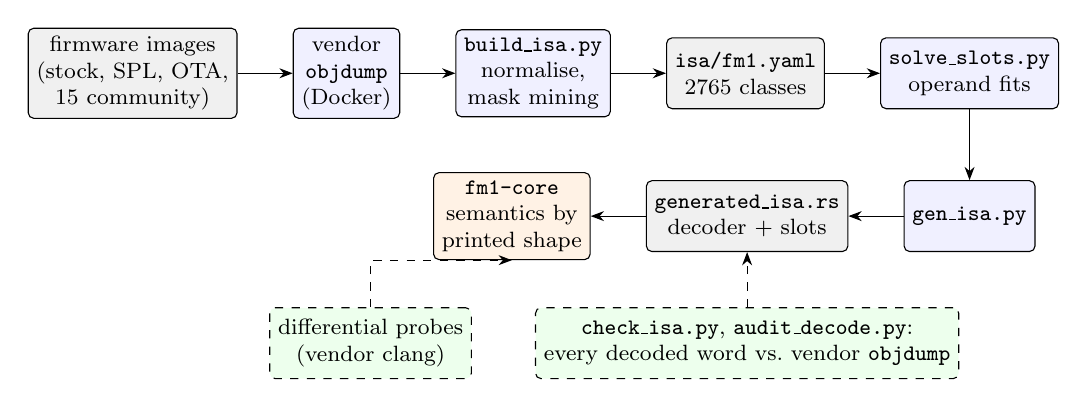
\begin{tikzpicture}[node distance=5mm and 7mm, >=Stealth,
  box/.style={draw,rounded corners=2pt,align=center,font=\footnotesize,minimum height=9mm,inner sep=3pt},
  data/.style={box,fill=black!6},
  tool/.style={box,fill=blue!6},
  chk/.style={box,fill=green!7,dashed}]
  \node[data] (fw) {firmware images\\(stock, SPL, OTA,\\15 community)};
  \node[tool,right=of fw] (od) {vendor\\\code{objdump}\\(Docker)};
  \node[tool,right=of od] (mine) {\code{build\_isa.py}\\normalise,\\mask mining};
  \node[data,right=of mine] (yaml) {\code{isa/fm1.yaml}\\2765 classes};
  \node[tool,right=of yaml] (solve) {\code{solve\_slots.py}\\operand fits};
  \node[tool,below=9mm of solve] (gen) {\code{gen\_isa.py}};
  \node[data,left=of gen] (rs) {\code{generated\_isa.rs}\\decoder + slots};
  \node[box,left=of rs,fill=orange!10] (core) {\code{fm1-core}\\semantics by\\printed shape};
  \node[chk,below=7mm of rs] (audit) {\code{check\_isa.py}, \code{audit\_decode.py}:\\every decoded word vs.\ vendor \code{objdump}};
  \node[chk,left=8mm of audit] (probe) {differential probes\\(vendor clang)};
  \draw[->] (fw)--(od); \draw[->] (od)--(mine); \draw[->] (mine)--(yaml); \draw[->] (yaml)--(solve);
  \draw[->] (solve)--(gen); \draw[->] (gen)--(rs); \draw[->] (rs)--(core);
  \draw[->,dashed] (audit)--(rs);
  \draw[->,dashed] (probe.north) |- (core.south);
\end{tikzpicture}
\caption{The ISA pipeline. The YAML table is the single source of truth: the Rust decoder is
generated from it and never edited by hand. Dashed: the checks that gate every regeneration.}
\label{fig:pipeline}
\end{figure}

\subsection{Mask mining from disassembly corpora}
The vendor \code{objdump} prints every instruction's bytes next to its text. Running it over five
corpora (the V13 and V14 applications, two bootloader builds and the USB OTA loader, about 421\,000
instructions) gives the raw material. \code{tools/build\_isa.py} normalises each line into a
\emph{printed shape}: registers become \code{R}, decimal and hex immediates \code{\#i} and
\code{\#h}, register lists are canonicalised, and the vendor's \code{<\_fw+0x...>} annotations are
stripped. (That last step had a costly bug: stripping un-anchored ate the \code{<} operator in
\code{ifs (r6 < 3) goto}, creating phantom forms that covered 3\,\% of the corpus. It is anchored at
the end of the line now.) Instructions with the same shape and length are grouped, and for each
group the bits that never vary become the class's \code{mask}/\code{match}.

The result on the first day was 1067 classes. A streaming decoder over the same corpora, choosing
by longest match, then mask popcount, then corpus count, decoded all of them with 0 mismatches and
0 undecodable words. When the fifteen community firmwares were added (their raw applications
wrapped in ELF for \code{objdump} by \code{tools/disasm\_app.sh}), the table was re-mined from 25
listings into 2765 classes; \code{tools/isa\_stable\_names.py} keeps class names stable across
re-mining because parts of the core key on them.

\subsection{Operand fields as exact linear models}
Masks say which bits are opcode; they do not say how the variable bits become operands. The first
operand fitter (\code{derive.py}) tried per-field templates and solved 206 classes. The approach
that worked, \code{tools/solve\_slots.py}, fits every printed operand of a class as an \emph{exact}
linear model over the class's varying bits, by rational Gaussian elimination, with collinear bits
resolved by a power-of-two search. Operand kinds are \code{imm}, \code{rel} (sign-extended, scaled,
pc-relative), \code{scaled}, \code{bit}/\code{nbit}, \code{composed}, \code{const}, \code{zero32} and
register blocks. A fit is accepted only if it reproduces \emph{every} sample of the class. This
raised coverage to 764 classes, 86.8\,\% of corpus instructions.

For instruction families whose encodings span several classes, \emph{family-level fitting} worked
best: take every corpus line of one printed shape across classes (e.g.\ all 5302
\code{if (rN op \#imm) goto} lines), propose the bit fields, and verify against all of them. Five
families went to zero mismatches in one session this way. Two examples of what came out:

\begin{itemize}
\item \textbf{Compare-immediate branches.} Register in bits 0--3; byte~1 selects the family
  (\code{f8} ==/!=, \code{f9} unsigned $\ge$/$<$, \code{fc} unsigned $>$/$\le$, \code{fd}/\code{fe}
  signed); bit~7 the second operator of the family; a 10-bit immediate assembled as
  bits(25,31)\,|\,bits(4,6)$\ll$7; offset $=2\cdot\mathrm{sext}_9(\ldots)$ from $pc+4$.
\item \textbf{The composed 12-bit immediate}, shared by \code{R = \#h}, \code{R = R op \#h} and
  memory read-modify-write forms. With code $c$ = bits(24,27) and $m$ = bits(16,23): $c=0$ is the
  literal $m$; 1 replicates $m$ per halfword; 2 places $m\ll8$ per halfword; 3 replicates per
  byte; $c\ge4$ is float-like, $E = 2c + (m\gg7)$, value $=(\mathtt{0x80}\,|\,(m\,\&\,\mathtt{0x7f}))\ll(32-E)$.
  This one rule reproduces a 70-entry table of observed constants (IEEE floats among them) and
  about 1650 ALU and move samples.
\end{itemize}

Bits the corpora never vary cannot be fitted from them. For those the \emph{assembler oracle} was
used: generate assembly text sweeping one operand at a time, assemble thousands of lines per Docker
run with the vendor Clang, and read the bytes back. This is how the FPU was found: the stock
firmware uses float instructions that \code{objdump} prints as \code{<unknown instruction>}; compiling
with \code{-mcpu=r3} and disassembling the assembler's output gave the \code{3f e5} encoding
(add, sub, mul, div, min, max, conversions).

\subsection{Semantics keyed by printed shape}
\code{fm1-core} executes instructions by their printed shape (\code{Cpu::exec\_syntax}), taking
operands from the generated slots in printed order, so one arm for \code{R = R + \#i} serves every
class that prints that way. Raw-bit decoders exist only where one class mixes encodings. When the
solver began covering a class, its hand-written decoder was deleted; three of those turned out to be
silently wrong (one stored \code{r9} instead of \code{r1} because it took bit~7 as part of the
register number). Behaviours established while booting real code include:

\begin{itemize}
\item \textbf{Dual-issue pairs}: an instruction printed with a trailing \code{\#} pairs with the next
  one, which reads registers from \emph{before} the first wrote them (deferred register commit).
\item \textbf{Predicated blocks} \code{if (rA op x) \{ \ldots\} else \{ \ldots\}} whose then/else
  lengths are counted in \emph{units} (a pair is one unit, a nested block one unit).
\item \textbf{Hardware loops} \code{rep N rR \{}: block length $2(\mathrm{bits}(4,7)+1)$ bytes,
  count in a register or immediate.
\item \textbf{Interrupt nesting} follows the Blackfin rule: an ISR can be interrupted only while its
  \code{reti} is saved on the stack. (Without this, a tick between an ISR's \code{reti} pop and its
  \code{rti} made the \code{rti} return to itself.)
\item \textbf{Two stacks}: in user mode an interrupt saves \code{sp} to \code{usp} and continues on
  \code{ssp}. The stock RTOS's context switch depends on it.
\item \textbf{Flags}: N, C (set means no borrow, as on ARM), Z, V in \code{psr}, read by Clang's 64-bit
  arithmetic right after the low-word add or subtract.
\end{itemize}

\section{Validation: how we knew it was right}

Without hardware, ``right'' had to be defined by things that could be checked mechanically. Four
methods were used, and every change had to pass the ones that applied.

\paragraph{1. Decoder audit against the vendor.} \code{tools/audit\_decode.py} decodes every word of a
vendor listing with the Rust decoder and compares operands with the vendor text. It found, for
instance, that a sp-relative pair store fitted on V13 alone broke for offsets $\ge 512$ (keys stayed
lit because LED arrays were stale).

\paragraph{2. Differential probes.} A probe is a small C program built with the vendor Clang in which
each check computes an expression at run time from \code{volatile} inputs and compares it with the
same expression folded at compile time by LLVM (Listing~\ref{lst:probe}). The compiler's constant
folder is thus the oracle for the compiler's own model of the ISA, and a mismatch is an emulator bug.
Probe suites cover integer arithmetic (121 checks), Felucca's Huffman font decoder on data from its
own packer (139), the FPU (1464 cases against LLVM's folding), and 64-bit and soft-double arithmetic.

\begin{lstlisting}[language=C,caption={From \code{probes/arith.c}. \code{T(runtime, folded)}: the
first argument compiles to pi32v2 instructions, the second to a constant.},label={lst:probe},captionpos=b]
volatile int32_t a = 1234567, b = -89, c = 7;
volatile uint32_t ua = 0xDEADBEEFu, uc = 13u;
T(a / c,  1234567 / 7);
T(b % c,  -89 % 7);
T(ua % uc, 0xDEADBEEFu % 13u);
T(a * 241, 1234567 * 241);
\end{lstlisting}

\paragraph{3. Same code, two machines.} Where a firmware's C source was available, a piece of it was
built both for the device and natively and compared word for word. X0X's TR-909 code exposed the
register-pair addressing modes (a pre-increment store overwrote one voice's settings with another's)
and a bitfield-extract instruction that had been executed as an add. Later, reSID's double-precision
setup computed on the emulator differed from the host; tracing it found that \code{psr} always read
0, so every 64-bit add lost its carry and every 64-bit subtract borrowed.

\paragraph{4. Byte-identical audio across execution modes.} The emulator has three ways to run the
same code: one instruction at a time (the reference), a block interpreter with micro-ops, and a JIT.
A bench mode (\code{fm1-live --bench MS} with \code{FM1\_BENCH\_WAV}, plus a scripted exercise of
every key, encoder and note) writes the raw audio. Every optimisation was accepted only if the audio
was byte-identical in all three modes \emph{and} to the build before the change, for every
firmware. This turns ``did the JIT break something subtle?'' into a file comparison. (Dual-core
firmwares are deterministic per mode but interleave cores at slightly different points, so for
them the comparison is per mode against the previous build.)

Table~\ref{tab:bugs} lists some of what these methods caught. Most bugs were invisible at the point
of failure: the symptom appeared much later, in a picture or a sound.

\begin{table}[t]
\centering\footnotesize
\begin{tabularx}{\textwidth}{@{}>{\raggedright}p{43mm}X>{\raggedright\arraybackslash}p{33mm}@{}}
\toprule
Defect & Symptom & Found by\\
\midrule
2-byte shift: bit 7 taken as register bit & CRT copy loops ran 4$\times$ too long; RAM corrupted & boot trace\\
\code{[R+\#i] = R}: bit 7 in source register & stored \code{r9} instead of \code{r1} & solver replacing hand code\\
16-bit read at word offset 2 & every 16-bit canvas sheared & probe (lcdtest)\\
unsigned compare immediates sign-extended & wrong branches on \code{if (r2 < 2111)} & probe\\
4-byte \code{R = R << \#n} run as \code{>>>} & wrong arithmetic in drawing code & probe\\
sp-relative pair offset $\ge 512$ & stale LED arrays, keys stayed lit & decoder audit\\
interrupt nesting & \code{rti} returned to itself; hang & live play\\
register-pair pre-increment modes & X0X's 909 settings overwritten & device vs.\ native build\\
\code{b4 e1} extract executed as add & an address used as an exponent & device vs.\ native build\\
no arithmetic flags & 64-bit add lost carry; reSID filter wrong & soft-double probes\\
random-number unit read as 0 & stock UI froze after 8\,s & debugging the freeze\\
unknown-access log shifted 8192 entries per access & one firmware ran far too slowly & investigating the slowdown\\
\bottomrule
\end{tabularx}
\caption{A selection of defects and how each was found.}
\label{tab:bugs}
\end{table}

\section{The system-on-chip}

\paragraph{Peripherals in boot order, lazily.} The SoC layer started with RAM, the XIP window and a
stub that logs every access to an unknown address and returns a benign value. The rule was:
\emph{the access log is the reverse-engineering roadmap}. A peripheral was modelled when a firmware
was seen to depend on it, from Felucca's HAL headers and the AC79 SDK where possible. In order:
the interrupt controller (priority nibbles, software latch, RAM vectors), TIMER4/TIMER5 on a
240\,MHz cycle clock, SPI NOR flash (fonts), an ST7789-style LCD on SPI1 with DMA, the I2S output
(ALNK0, double-buffered DMA; Felucca's samples turned out to be 24-bit words in the \emph{low}
bits, not left-justified as a HAL comment says), the SAR ADC (MASTER pot, battery), and the key
matrix behind two 74HC595 shift registers with seven quadrature encoders.

\paragraph{Felucca first, then the stock firmware.} Felucca (open source) ran end to end on day
three. The stock firmware needed more, each piece found from a concrete symptom: SPI2 DMA to scan the
key columns (keys ignored), a hardware lock between cores for \code{lockset}/\code{lockclr} (a task
queued twice), a CRC-16 unit (the patch file system failed every CRC), \code{idle} that waits for an
interrupt (0.44$\times$ real time), and a random-number generator: a routine in the audio driver
parks its task when a random word equals a fixed descrambled value, which a constant 0 always did,
so the UI froze about eight seconds after boot. The factory DX7 patch bank lives in a flash area
that updates never write; since it cannot be redistributed, a blank area gets the emulator's own
small bank, and \code{--syx} loads a DX7 bank.

\paragraph{Two cores.} The stock firmware renders sound on core 1. Core 1 starts when core 0 sets a
bit at \code{0x10008} (latched at the write: some firmwares hold it only briefly), at the address in
\code{0x01C7FFF8}. It has no clock of its own: core 0 runs in slices of 1024 instructions, then core
1 runs as many instructions as cycles passed, and stops early when it returns to the same pc with
the same registers (a job loop with nothing to do).

\section{Making it fast}

FM-1 firmwares do their audio in an interrupt every 128 samples, and live play needs the full
240\,MHz in real time. Speed was added in stages, each gated on the byte-identical audio rule:

\begin{enumerate}
\item \textbf{Decode cache} and cheap shape matching: from 1\,M to 17\,M instructions/s.
\item \textbf{Micro-ops and blocks}: common forms pre-decoded with operands and branch targets
  resolved once; straight-line blocks; RAM/XIP fast paths; idle skipping of timer-polling loops.
  Interrupt delivery stays exact at block granularity: blocks end at due ticks, peripheral writes,
  and the ends of pairs, predicated blocks and loops.
\item \textbf{AArch64 JIT} (macOS): hot blocks compiled to native code with chaining, guest state
  in the \code{Cpu} struct, inline RAM/XIP loads and stores, helpers that sync the clock to the exact
  instruction for everything else.
\item \textbf{Shrinking the slow path}: 1.7--3.8\,\% of instructions fell back to the generic path
  and cost half the time, because each also ended a block. New micro-ops (shared with the
  interpreter through one \code{exec\_raw}, so the two cannot drift), dual-issue pairs with no
  dependency run as two plain ops, and a remembered ``needs step'' marker brought it to 0.1\,\%.
\item \textbf{WebAssembly JIT}: in the browser, a hot block's \emph{region} (blocks reachable over
  fixed edges, at most 32 blocks or 384 ops) becomes a small Wasm module that the host compiles and
  installs in the exported function table; Rust calls it by index. Per-block modules gained nothing
  (blocks average 3.5 instructions); regions doubled the speed. Chrome compiles them synchronously
  inside the AudioWorklet in about 25\,\textmu s, at most 16 per audio quantum.
\end{enumerate}

\begin{table}[h]
\centering\footnotesize
\begin{tabular}{@{}lccc@{}}
\toprule
Real-time factor at 240\,MHz & slowest (X0X) & Felucca & fastest (Melodee)\\
\midrule
native, AArch64 JIT & 1.14 $\rightarrow$ 2.65 & 1.63 $\rightarrow$ 4.4 & 3.1 $\rightarrow$ 5.9\\
WebAssembly (Node) & 0.53 $\rightarrow$ 1.62 & 0.66 $\rightarrow$ 2.3 & 0.97 $\rightarrow$ 3.5\\
\bottomrule
\end{tabular}
\caption{The speed pass of day four (before $\rightarrow$ after); every firmware's bench audio
byte-identical to before.}
\label{tab:speed}
\end{table}

One measure that was tried and dropped: per-block tick accounting in the interpreter, paid before
any non-RAM access. It was 5--7\,\% slower, because blocks are short. A/B timing was done
interleaved (\code{tools/bench\_ab.sh}), since back-to-back runs drifted 6--8\,\%.

\section{The browser, MIDI and publishing}

The web build runs the emulator in an AudioWorklet. The page hosts no firmware: it fetches each
update package from its author's GitHub Pages (all allow cross-origin reads) and unpacks it with
\code{web/fwsc.js}, a package reader checked byte-equal against Felucca's own on every package.
Authors publish new versions often; when the catalog's URL is gone, the page takes the package the
author's installer page names now (four had moved on the day of publication). M-VAVE's server sends
no CORS header, so users open their own copy of the stock package.

New versions also test the emulator. On the day this report was written, Felucca~1.6 appeared and
the page picked it up; the emulator halted on \code{d7 ec 51 38}, which the vendor prints as
\code{[r5+-128] = r3}. The table had a class for it with 19 samples but no operand fit. Comparing
all word loads and stores in the 25 listings showed that bit~17 selects pre-increment or a plain
offset and that byte~0's bit~2 is the offset's sign: one model, 27\,884 samples, 0 mismatches. With
it Felucca~1.6 plays, and every other firmware's audio stayed byte-identical.

MIDI~IN is modelled at the UART, not injected into firmware: UART1 with receive DMA into a ring, a
latch that counts received bytes, and a timeout interrupt after a configured silence, one byte per
31\,250-baud byte time (320\,\textmu s). Each firmware therefore reads MIDI with its own driver;
Felucca polls the count from a timer interrupt, the stock firmware takes the timeout interrupt. The
emulator found that the stock firmware listens on channel~2, a claim still to be checked on a real
unit. In the browser, Web MIDI feeds the bytes; natively, every MIDI input of the computer.

Continuous integration runs the unit tests, builds the site and runs two smoke tests in Node
against the built WebAssembly: Felucca must boot to a screen and sound and play a MIDI note; the
SID firmware must stay silent until a key is pressed, then sound. The project began inside a
larger repository of demos and was moved into its own repository with history kept
(\code{git subtree split}); the old URLs forward with their query strings.

\section{A new firmware, developed on the emulator: FM-1 SID}

To test the emulator as a development platform, we asked whether the FM-1 could be a Commodore~64
SID synth. The study (Table~\ref{tab:sid}) compared an integer SID model written for the purpose
with reSID~0.16, reSID~1.0 and reSIDfp, by recording register streams and replaying them on every
engine, each clocked to the exact cycle of each write; the costs on the FM-1 were measured by
counting emulated instructions between markers, and the FM-1 output was compared with the host
build of the same code (bit-identical in every case).

\begin{table}[h]
\centering\footnotesize
\begin{tabular}{@{}lrrl@{}}
\toprule
Engine & instr./sample & of a 240\,MHz core & verdict\\
\midrule
own integer model & 316 & 5.8\,\% & fits; lowest fidelity\\
reSID 0.16, fast & 440 & 8.1\,\% & \textbf{fits; chosen}\\
reSID 0.16, interpolate & 5\,562 & 102\,\% & too heavy\\
reSID 0.16, resample & 39\,226 & 721\,\% & far too heavy\\
reSID 1.0 / reSIDfp & -- & -- & 8--21\,MB filter tables; FM-1 has 1\,MB flash\\
\bottomrule
\end{tabular}
\caption{SID engines per chip (3 voices and filter) at 44.1\,kHz, measured on the emulated FM-1.}
\label{tab:sid}
\end{table}

The firmware that followed nests machines: a C64 tune's own 6502 code runs in floooh's cycle-stepped
\code{m6502.h}, compiled for pi32v2, which runs on the emulated FM-1, which runs in WebAssembly in the
browser, whose hot pi32v2 code is compiled at run time into further WebAssembly. The main loop runs
the tune's play routine up to three frames ahead and queues each SID write with its C64 cycle; the
audio interrupt clocks reSID to each write's cycle. Output correlates 0.984 with host reSID fed the
same stream. The web page searches all 61\,157 tunes of the High Voltage SID Collection, fetched
from \code{hvsc.c64.org} when picked and appended to the firmware image as a ``tune pack''.

The firmware then grew into an instrument: a synth mode where the keys play twelve SID patches, a
three-track step sequencer, and an effects page (Fig.~\ref{fig:fx}) with stereo chorus, a tempo
delay whose right tap answers 1.5 times later, and a room reverb (four damped combs, two allpasses),
adapted from Felucca's effects. The same verification style applied: with effects at zero the
player's output was compared sample by sample with the firmware before the change (0 of 176\,512
samples differed); the audio interrupt's load rose from about 10\,\% to 14\,\% of the core, and RAM
use to 425 of 432\,KB. The firmware is packaged as a real FM-1 update package with Felucca's update
loader and three hash-checked files of JieLi's Apache-licensed SDK, and the package boots straight
into the synth mode. The firmware image, rebuilt on macOS through the Dockerised toolchain, was
byte-identical to the one built on Linux.

Writing this firmware found four more emulator defects (the flags and carry gaps of
Table~\ref{tab:bugs} among them), which is itself an argument for developing against an emulator
whose every fix comes with a probe.

\begin{figure}[t]
\centering
\includegraphics[width=0.36\textwidth]{fig/fxpage.png}
\caption{FM-1 SID's effects page on the emulated LCD: the knob assignments, the delay time computed
from the sequencer tempo, the chip model, and an oscilloscope of the output.}
\label{fig:fx}
\end{figure}

\section{Tuning towards the real hardware}
\label{sec:hw}

\paragraph{Released before it was tested.} FM-1 SID was offered for download as an FM-1 update
package on 11 October, a day after the first community firmware ran on the emulator, and for a few
days the community's firmware hub listed it beside firmwares that had run on real units. Nobody on
the project owned an FM-1 yet. Eight days later, people who installed it found that it played but that their computers no longer
saw the synth (GitHub issues \#22 and \#24, 19 October): FM-1 SID had no USB stack at all, and an
FM-1 firmware is updated only through the firmware that is running, so no installer could reach it.
The way back was found by the community, not by us: holding OCT$-$ and OCT$+$ together for about five
seconds at power-on enters the chip's own update mode, below every firmware, from which a third-party
flasher (M-flasher) wrote M-VAVE's stock firmware back. FM-1 SID was taken off the hub. No unit was
damaged permanently, but each owner had to find and perform that recovery themselves.

The emulator could not have caught this. It had no USB model then (one was added after the hardware
arrived), and nothing in it asked whether a firmware can be replaced. The
failure was one of process rather than emulation: a firmware that had never run on hardware was
published as an install. The rule taken from it: what has not run on a real FM-1 is labelled so, and
a package is offered only once it has run there, with its way back tested on the device.

\paragraph{Round one: the emulator was not the device.} The FM-1 arrived on 23 October, and the
first attempt to fix FM-1 SID on it was humbling. USB-MIDI was added, with three exits to the update
mode (OCT$-$ and OCT$+$ held while running, two failed starts in a row, and the installers' upgrade
command), and every check on the emulator passed. On the device, the synth mode played but no tune
did, and the firmware received the installer's commands but none of its replies reached the
computer. Getting the unit back took three recoveries through the chip's mask-ROM mode, for which no
macOS tool exists (a Linux machine and MvaveFM1Unbricker). The question was no longer ``is the
emulator consistent?'' but ``where does it differ from the chip?''.

\paragraph{fm1-dock: install once, then deploy and measure.} The day after the first reports of stuck
units, three days before the hardware arrived, the author asked whether the risk could be removed at its
source: a thin resident layer, installed once, through which experimental synths are deployed and
inspected without a full firmware upgrade each time. That layer was built on the emulator as
\emph{harbor} and renamed \emph{fm1-dock} when it was released. It is a host firmware, grown from
zvenson's Dinghy, that owns everything a broken experiment must not take down: USB-MIDI, the
installers' protocol, the USB rescue (OCT$-$ at power-on), the screen and the keys. Over its own
SysEx commands it accepts three kinds of code. A \emph{module} is a synth, compiled against a small
host interface, written into a flash slot fm1-dock reserves for it (a deploy takes about ten
seconds, erases only that slot, and can be undone by deleting the module), and picked with HOME.
A \emph{probe} is a program relocated into RAM and run once; nothing is written to flash. A file sent
to the running module's \code{data()} hook (the MODULE command) is how FM-1 SID 0.3 plays a tune sent
over USB, straight into its emulated C64's memory. The emulator speaks the same protocol over an
emulated USB device, so every tool runs unchanged against either machine.

\paragraph{Measuring instead of guessing.} The probes were what answered the question. A probe writes
typed records (numbers, words, TIMER4 timings with the interrupts off and an empty loop subtracted)
into a buffer in memory that survives a reset, so a probe that crashes still reports how far it got
and where. The same probe runs on the FM-1 and on the emulator (\code{tools/probe.py run X.c --on
emu,fm1}), and the two results are printed side by side with the ratio of every timing. A new
question about the hardware costs a C file of a few dozen lines and a few seconds, not a firmware
install and a risk to the unit; Table~\ref{tab:probes} lists the questions asked in the first two
days.

The first probe found the first gap. Every probe crashed on the device on its second instruction,
at the same addresses each time, while the emulator ran them happily. Reading the crash record
(another probe, a memory dump) showed the CPU exception with cause bit~12 of the debug unit: the
\emph{PC limit}. Dinghy's start-up code, inherited from Felucca, arms the core's guards: instruction
fetches are allowed only within the firmware's own code and its RAM routines, writes into the stack
guard bands and the vector area trap, and so do accesses to unmapped space. The emulator modelled
none of this. With the guards modelled (the limit registers kept, a block fetched outside both
windows ends a run, the instruction executes and interrupt~1 is raised with the cause set), the
emulator crashed the same probes at exactly the device's addresses, \code{0x01C301A2} and
\code{0x01C301BA}. With fm1-dock widening the PC limits around a probe, both ran: the first program
loaded and run from RAM on a real FM-1.

\paragraph{What the probes measured.} Table~\ref{tab:hw} lists the gaps found, each turned into an
emulator change and a test. Three of them explained FM-1 SID's failure on the device. The emulator
finished LCD transfers at once, while the real SPI clock is about 11\,MHz: FM-1 SID redrew the whole
screen (115\,KB, $\approx$82\,ms) every 40\,ms and waited for it, which starved the main loop that
runs the tune ahead of the audio interrupt. With timed LCD transfers the emulator reproduced the
silence (peak level 112 instead of 9\,086) and now warns when the screen takes most of the time.
The second was speed: the emulator charged one 240\,MHz cycle per instruction, but FM-1 SID's own
load meter read 24\,\% on the device against 13\,\% on the emulator. Emulated at 130\,MHz, the
emulator reproduced the device exactly (GoatTracker songs played, an RSID tune went silent), and
the cause was a firmware bug that only a slow enough CPU exposes: once the play routine fell behind
the audio interrupt, an unsigned \code{gen\_cyc - play\_cyc} wrapped and generation stopped for
good. The third, the installer that never answered, is still not explained; one plausible theory
(the \code{idle} instruction in the main loop) was refuted by a probe that sent 40 MIDI notes over
USB between \code{idle}s and saw all 40 arrive.

\begin{table}[t]
\centering\footnotesize
\begin{tabularx}{\textwidth}{@{}>{\raggedright}p{36mm}X>{\raggedright\arraybackslash}p{36mm}@{}}
\toprule
Gap & On the FM-1 & In the emulator now\\
\midrule
LCD transfer time & SPI $\approx$11.2\,MHz; a full frame $\approx$82\,ms & timed at 12\,MHz; a warning when the screen dominates\\
PC limit, bus guard & a fetch outside the limits, or a NULL-page access, raises the exception & modelled, cause bits in \code{DBG\_MSG}\\
Misaligned 16/32-bit RAM access & faults (\code{EMU\_MSG} bit 0, always on); flash reads across bytes & faults in strict mode\\
Instruction cost & 0.58--6.75 cycles by class (Table~\ref{tab:cyc}) & per-class costs in strict mode\\
Flash cache & 32\,KB, 64-byte lines, $\approx$300 cycles a miss & modelled in strict mode\\
TIMER4 & 24\,MHz to 51\,ppm against the host's USB frames & as assumed\\
\code{trigger} (fault stub) & freezes the trace unit & a no-op (was ``unsupported'')\\
\bottomrule
\end{tabularx}
\caption{Differences between the emulator and the FM-1 found with probes, and what was done.}
\label{tab:hw}
\end{table}

\paragraph{A cycle model.} A probe with one instruction per statement (inline assembly, eight per
loop round) gave the cost of each instruction class on the device (Table~\ref{tab:cyc}). The core is
fast at straight-line arithmetic, which it issues two at a time, and slow at control flow: a taken
branch costs five to six cycles, a call and return ten. A second probe swept the footprint and stride
of flash reads: a footprint up to 32\,KB hits, 64\,KB misses; the cost doubles with the stride up to
64 bytes; a miss costs about 1.3\,\textmu s. These numbers became a \emph{strict} mode
(\code{FM1\_STRICT=1}): the interpreter only, a clock in eighths of a cycle, each instruction its
measured cost (taken and not-taken branches apart), a 32\,KB, 64-byte-line cache in front of flash
for data and code, and misaligned accesses faulting. In strict mode FM-1 SID's load meter reads
21\,\% (device 24\,\%, fast mode 13\,\%), every class of Table~\ref{tab:cyc} but the load-use stall
is within about 10\,\% of the device (a store followed by a load of the same word, and independent
multiplies, are not modelled either), and the firmware build that failed on the device fails the
same way. The fast modes still count one cycle per instruction: changing the three
compilers' accounting is left for later.

\begin{table}[t]
\centering\footnotesize
\begin{tabular}{@{}lrrlrr@{}}
\toprule
Instruction class & FM-1 & strict & Instruction class & FM-1 & strict\\
\midrule
\code{nop}, \code{and}, add & 0.58--0.75 & 0.62 & load word / half / byte & 1.25--1.34 & 1.25\\
6-byte constant & 1.08 & 1.12 & store & 1.42 & 1.45\\
multiply & 1.92 & 1.88 & push + pop of 4 registers & 10.6 & 10.5\\
divide & 6.75 & 6.78 & \code{goto} & 5.17 & 5.25\\
branch, not taken & 0.85 & 0.88 & branch, taken & 6.50 & 6.50\\
call + return & 10.2 & 10.0 & load feeding a load & 3.08 & 1.25\\
\bottomrule
\end{tabular}
\caption{Cycles (240\,MHz) per instruction measured on the FM-1 (\code{probes/cycles.c}, run from
RAM) and charged by the emulator's strict mode. The load-use stall in the last row is not modelled
yet.}
\label{tab:cyc}
\end{table}

\paragraph{DSP, the FPU, and what the community uses.} The same method looked at the core's DSP-style
instructions. Halfword multiply-accumulates with saturation cost 1.2 cycles on the device, three times
less than the 64-bit multiply-accumulate chain the compiler emits for \code{acc += (int64\_t)a * b}
(3.4 cycles); the saturating shift exposed as \code{\_\_builtin\_pi32v2\_qasl} clamps in 0.6 cycles; a
cache line prefetch (\code{pfetch}) issued a microsecond ahead halves a miss. A probe of audio
kernels, run on both machines with checksums of the output, showed that a biquad costs about 20
cycles a sample in any form (32-bit, 64-bit MAC, halfword MAC, or single-precision float on the
hardware FPU), and that a float state-variable filter is faster than its integer version; every
checksum the emulator could compute matched the device's. The probe also exposed a limit of corpus
mining: the halfword multiply-accumulate classes were fitted only for the register combinations the
corpora contain, so the emulator cannot decode them with any others. Running all 80 published
firmwares on the emulator with an executed-instruction histogram showed that none uses those
instructions, a few use 64-bit multiplies, and 16 do a substantial part of their work on the FPU.

The cost of a filter turned out not to lie in its arithmetic but in its loop: the taken branch that
closes an iteration costs as much as six plain instructions. The core has hardware loops,
\code{rep N rR \{ \ldots\ \}}, which no firmware's compiler emits (the 80 firmwares executed eight
between them). Probes established three rules that no document states: the body is at most 32 bytes
(the assembler counts it), the loop counts its register down to zero, and only counts up to 31 work
(for 32 and above the device runs the count modulo 32, plus one, times; the emulator ran the full
count, the one semantic error the probes found). Within those rules, a hardware loop with halfword
multiply-accumulates runs a 64-tap FIR on 16-bit samples at 2.9 cycles a tap against 11 for the C
loop, 3.9 times faster, with an identical result (Table~\ref{tab:dsp}): one channel at 44.1\,kHz goes
from 13\,\% of the core to 3.4\,\%. The gain is in tight inner loops (FIR, multi-tap delays, mixing,
gain); a biquad's body does not fit 32 bytes. One hoped-for gain did not exist: the emulator's map has
a 512\,KB ``overlay'' bank at \code{0x04000000} and 256\,KB at \code{0x01F00000}, guessed on day one, but
on the device the first hangs the bus, the second faults (the stock start-up clears 16\,KB there after
writing cache control registers: most likely the cache's own memory), and so does anything past the
512\,KB of main RAM.

\begin{table}[t]
\centering\footnotesize
\begin{tabular}{@{}lrrr@{}}
\toprule
Kernel (on the FM-1) & C & hardware loop + DSP & speed-up\\
\midrule
loop overhead (a load and an add an iteration) & 6.75 & 2.38 & 2.8$\times$\\
64-tap FIR, per tap (C with a 64-bit accumulator: 9.78) & 11.06 & 2.86 & 3.9$\times$\\
block gain with a clamp, per sample & 12.81 & 5.70 & 2.2$\times$\\
\bottomrule
\end{tabular}
\caption{Cycles on the FM-1 (\code{probes/dspx2.c}): C as the vendor compiler builds it, against
inline assembly with a hardware loop (\code{rep}), halfword multiply-accumulates with saturation and
the saturating shift. Every fast version gives the C version's result.}
\label{tab:dsp}
\end{table}

\begin{table}[t]
\centering\footnotesize
\begin{tabularx}{\textwidth}{@{}>{\raggedright}p{50mm}X@{}}
\toprule
Question (probe) & Answer on the FM-1\\
\midrule
Does code run from RAM? (the first probe) & No: it faults on its second instruction (the PC limit); it runs once fm1-dock widens the limits\\
Does \code{idle} in a main loop stop USB? (\code{idle}) & No: 40 of 40 MIDI notes sent between \code{idle}s, each $\leq$93\,\textmu s\\
Must a USB transmit buffer be 8-byte aligned? (\code{usbtxoff.c}) & No: fm1-dock's driver sends from offsets 4 and 12, although that rule fitted all six failed FM-1 SID builds in the emulator\\
Can a probe drive a USB endpoint itself? & Not safely: the computer stopped collecting from the FM-1 until a replug; probes send through fm1-dock\\
Misaligned 16/32-bit RAM access (\code{align}) & Faults, always\\
LCD SPI clock (\code{lcd}) & $\approx$11.2\,MHz: a full frame takes $\approx$82\,ms\\
TIMER4 against the computer's USB frames (\code{clock}) & 24\,MHz within 51\,ppm\\
Instruction costs (\code{cycles.c}) & 0.58--10.6 cycles by class (Table~\ref{tab:cyc})\\
Flash cache (\code{cache.c}) & 32\,KB, 64-byte lines, $\approx$300 cycles a miss\\
Hardware loops, DSP instructions (\code{dspx2.c}) & body $\leq$32 bytes, counts $\leq$31; FIR 3.9$\times$ faster (Table~\ref{tab:dsp})\\
Memory banks mapped since day one & \code{0x04000000} hangs the bus, \code{0x01F00000} faults\\
\bottomrule
\end{tabularx}
\caption{Questions answered by probes run from RAM through fm1-dock on 24--25 October. Each took a
C file and seconds on the device; none wrote flash.}
\label{tab:probes}
\end{table}

\paragraph{Round two: let the host own USB.} The probes refuted the two theories for FM-1 SID's silent
USB: \code{idle} was not it, and neither was buffer alignment, although an emulator rule requiring it
reproduced every failed build. A rule fitted to past failures is not evidence until the chip agrees.
Rather than keep hunting the bug in FM-1 SID's own USB code, FM-1 SID was rebuilt as an fm1-dock
module, so that fm1-dock answers the installers whatever the module does. The probes' findings went
in at the same time: the screen sends only the rows that changed, a strip at a time with the tune fed
between strips; a play routine that falls behind catches up instead of stopping; and the
cycle-stepped 6502 core gave way to one that runs an instruction per dispatch with each memory access
at its cycle, fast enough for the slower real CPU (PSID output bit-identical, RSID checked against
libsidplayfp). Deployed the same day, it played on the device and USB answered while it played.

\paragraph{Round three: the safety net is hardware too.} The standalone FM-1 SID was then deployed into
a developer feature of fm1-dock, a \emph{boot slot} that fm1-dock hands the FM-1 to at power-on, to
study its USB bug on the chip. Two flaws made it a trap. fm1-dock decided to hand over by comparing
names, and the boot firmware had the same name as the selected module. And the escape keys were read
only in the first 50\,ms after power-on, which the emulator honoured and the device did not. Every
start handed over to the firmware whose USB was broken, and the unit needed a fourth recovery from
Linux. The fixes: release builds have no boot slot at all (a boot firmware is refused, an old entry is
forgotten at start-up), the power-on keys are read for 500\,ms, and OCT$-$ is read again while
fm1-dock starts. The lesson is the section's in miniature: a rescue path is hardware behaviour, and
it is not proven until it has been taken on the device.

\paragraph{Round four: released, verified on the device.} On 25 October FM-1 SID 0.2 shipped as a
solo firmware built on fm1-dock: one module, with fm1-dock's USB, installer protocol and rescue
underneath. It was installed with a community installer and played with the heaviest audio block at
34\,\% of its time and no overruns, while the installers reached it over USB. The same evening
fm1-dock 0.6 and FM-1 SID 0.3 added two features that need the device and the browser together: any
SID tune picked on the web page is sent over USB into FM-1 SID's emulated C64 memory and plays at once
(Commando in 1.6\,s, nothing written to flash), and the FM-1's keys go out as MIDI notes, so the real
FM-1 plays the emulated one in the browser. Table~\ref{tab:rounds} summarises the rounds.

\begin{table}[t]
\centering\footnotesize
\begin{tabularx}{\textwidth}{@{}l>{\raggedright}p{52mm}X>{\raggedright\arraybackslash}p{24mm}@{}}
\toprule
Date & Change & On the FM-1 & Recoveries\\
\midrule
11--19 Oct & FM-1 SID package, tested on the emulator only; no USB & plays; no computer sees it & owners, chip's mode + M-flasher\\
23 Oct & USB-MIDI, three exits to the update mode & tunes silent; installer replies never arrive & 3, from Linux\\
24 Oct & probes on fm1-dock; screen strips, catch-up, a faster 6502 core; FM-1 SID as a module & plays; USB answers while it plays & --\\
25 Oct & the standalone in fm1-dock's boot slot, to study its USB & escape keys missed; handed over at every start & 1, from Linux\\
25 Oct & no boot slot in releases, longer key reads; FM-1 SID 0.2 as a solo app & heaviest block 34\,\%, no overruns; installers answer & --\\
25 Oct & fm1-dock 0.6, FM-1 SID 0.3: tunes over USB, keys as MIDI & a tune from the page plays on the device in 1.6\,s & --\\
\bottomrule
\end{tabularx}
\caption{FM-1 SID from its first release to one verified on the device.}
\label{tab:rounds}
\end{table}

\paragraph{What changed.} The emulator was right about almost everything that its oracles could
reach: of everything the probes tested, one instruction's semantics needed correcting (the hardware
loop's count), and every kernel it could run gave the device's output. It was wrong about what no
oracle covered: timing, caches, and the protections a start-up file switches
on. Those are exactly the things a vendor disassembler and a compiler's constant folder cannot know,
and a day of probes on the device measured them. The rule we take from it is the one
the probe tool makes cheap: a claim about the hardware is a measurement, and a firmware is not ready
for the device because it passes on the emulator, but because the emulator has been shown to fail
the way the device fails.

\section{How the work was organised}

\begin{table}[t]
\centering\footnotesize
\begin{tabularx}{\textwidth}{@{}lX@{}}
\toprule
Day & Result\\
\midrule
1 (Oct 8) & Recon; toolchain verified in Docker; V13 disassembly reproduced byte-for-byte.\\
2 (Oct 9) & 1067 classes mined, operand solver (86.8\,\% of instructions); stock V13 boots to RTOS start on two cores.\\
3 (Oct 10) & Interrupts, timers, flash, LCD, I2S, keys: Felucca plays; live at 240\,MHz with the AArch64 JIT; fifteen firmwares, the FPU, the browser build, published.\\
4 (Oct 11) & Flags and carry; stock firmware with both cores; SID study, player firmware, HVSC page, synth mode, update package, sequencer; WebAssembly JIT.\\
5 (Oct 12) & MIDI in; a guide on the page; own repository; FM-1 SID boots as a synth, with effects.\\
Oct 19--20 & Users who installed FM-1 SID cannot reach their FM-1 over USB; the community finds the way back. The idea of a host to deploy synths into.\\
Oct 23--24 & The FM-1 on the desk: FM-1 SID fails on it; fm1-dock and probes over USB-MIDI; guards, timed LCD, a cycle and flash-cache model; FM-1 SID as an fm1-dock module (Section~\ref{sec:hw}).\\
Oct 25 & A boot-slot trap and its fixes; fm1-dock 0.6 and FM-1 SID 0.2 and 0.3 released, verified on the device.\\
\bottomrule
\end{tabularx}
\caption{Timeline. Each commit is a working state that passed the checks.}
\label{tab:time}
\end{table}

The work was done by one person directing an AI coding agent (Claude Code, Anthropic). The division
of labour was roughly as follows. The human chose what to build and in which order (the emulator
itself, the SID synth idea, adding effects, booting the SID firmware as a synth, moving to a
repository of its own), judged results by playing and listening, decided the tone of the public
pages (``a better story'', less technical), and approved anything outward-facing: pushes, publishing,
messages to others. The agent read the sources, ran the vendor toolchain, wrote the mining and
fitting tools, the emulator, the probes and the firmware, measured, and kept a running work log
(\code{PLAN.md}) that recorded each phase's state, numbers and open questions, so that work could
resume after an interruption or in a new session. Separate agents were occasionally used for
self-contained jobs, such as writing the page's guide.

What made the agent's output trustworthy was not review of every line but a small set of rules that
turned claims into checks:

\begin{itemize}
\item \textbf{One source of truth.} The decoder is generated from the YAML table; a second,
  hand-maintained table was never allowed. When generated slots covered a class, the hand-written
  decoder was deleted, which is how three silent bugs surfaced.
\item \textbf{The oracle is the vendor, not a guess.} Encodings are checked against the vendor
  disassembler; semantics against the vendor compiler's constant folding; unseen bits against the
  vendor assembler.
\item \textbf{Byte-identical or it did not happen.} Optimisations must leave audio unchanged across
  execution modes and against the previous build, for every firmware.
\item \textbf{Log the unknown, never swallow it.} Unknown memory accesses are logged, unknown
  instructions halt with their class name; both are to-do lists.
\item \textbf{State what is unverified.} Statements not yet checked on hardware (the stock MIDI
  channel, FM-1 SID on a real unit, which instructions set flags) are marked as such in the
  documentation and on the pages.
\item \textbf{The device decides, and the way back comes first.} Learned late, from FM-1 SID's first
  users (Section~\ref{sec:hw}): an emulator pass makes a firmware a candidate, not a release. Nothing
  is offered for install before it has run on a real FM-1, and nothing risky goes onto the unit
  before its way back has been taken on the chip itself. Installs on the unit are run by the human;
  the agent may read from the device (identity, logs) and run probes, which never write flash.
\end{itemize}

\section{Limitations}

Section~\ref{sec:hw} compares the emulator with a real FM-1, but only in part. Instruction costs and
the flash cache are modelled in the strict mode only; the fast modes still charge one cycle per
instruction, and load-use and store-to-load stalls, sequential prefetch and a possible split of the
cache between code and data are not modelled. The write and stack limits of the guards are not
modelled, and misaligned accesses fault only in the strict mode. Why the standalone FM-1 SID builds never
answered an installer on the device is not explained; FM-1 SID avoids the question by leaving USB to
fm1-dock. In the emulator about one USB command frame in 80 is lost after the device has accepted
its packets, so the senders repeat a frame after a second; whether the device does the same is not
measured. Which instructions update flags on the real
core is still assumed from compiled code, which only reads them right after a producer. Two FPU
operations in the stock firmware (codes 7 and 8) are unknown, the halfword multiply-accumulate
classes decode only for the register combinations seen in the corpora (656 classes in all have no
solved operand fields), the hardware loop still runs counts of 32 and more in full, the two memory
banks that do not exist on the device are still mapped, and the real entry chain of
core 1 is not understood; the emulator starts it at the address the firmware writes. Each of these
is now a probe away from a measurement.

\section{Conclusion}

An undocumented CPU in a consumer device turned out to be recoverable from its firmware in days,
because the vendor's own tools could serve as oracles: the disassembler for encodings, the assembler
for bits the corpora never vary, and the compiler's constant folding for semantics. The rest was
engineering discipline: a generated decoder, peripherals modelled on demand from an access log, and a
byte-identical audio rule that let aggressive optimisation (two JITs) proceed without fear. The
result runs every published FM-1 firmware in a browser, and was good enough to develop a new
firmware on before the synth was on the desk.

\section*{Acknowledgements}
Built on the community's work: AL-255's FM-1-RE, ip2k's lunar-modulator, kagaimiq's jielie,
hugelton's Felucca (whose hardware layer and effects FM-1 SID uses), cicloid's awesome-fm-1, and every
firmware author who published their work. reSID is by Dag Lem; \code{m6502.h} by Andre Weissflog;
the SID tunes come from the High Voltage SID Collection.

\begin{thebibliography}{9}\small
\bibitem{fm1re} AL-255. \emph{FM-1-RE}. \url{https://github.com/AL-255/FM-1-RE}
\bibitem{lunar} ip2k. \emph{lunar-modulator}. \url{https://github.com/ip2k/lunar-modulator}
\bibitem{jielie} kagaimiq. \emph{jielie}. \url{https://kagaimiq.github.io/jielie}
\bibitem{felucca} hugelton. \emph{Felucca}. \url{https://github.com/hugelton/Felucca}
\bibitem{awesome} cicloid. \emph{awesome-fm-1}. \url{https://github.com/cicloid/awesome-fm-1}
\bibitem{resid} D.~Lem. \emph{reSID}, version 0.16.
\bibitem{chips} A.~Weissflog. \emph{chips} (\code{m6502.h}). \url{https://github.com/floooh/chips}
\bibitem{hvsc} \emph{High Voltage SID Collection}. \url{https://hvsc.c64.org}
\bibitem{emu} J.~Eriksson. \emph{fm1-emu}. \url{https://github.com/joakimeriksson/fm1-emu}
\end{thebibliography}

\end{document}
